\documentclass{acm_proc_article-sp}
\usepackage[utf8]{inputenc}
\usepackage{url}
\usepackage{listings}
\usepackage{color}
\usepackage{graphicx}
\graphicspath{{./imagens/}}
 
\definecolor{dkgreen}{rgb}{0,0.6,0}
\definecolor{gray}{rgb}{0.5,0.5,0.5}
\definecolor{mauve}{rgb}{0.58,0,0.82}
\definecolor{dkblue}{rgb}{0,0,.6}
\definecolor{dkyellow}{cmyk}{0,0,.8,.3}

\begin{document}

\title{Utilizando SOAP para construir Web Services}
%\titlenote{(Does NOT produce the permission block, copyright information nor page numbering). For use with ACM\_PROC\_ARTICLE-SP.CLS. Supported by ACM.}}
%\subtitle{[Extended Abstract]
%\titlenote{A full version of this paper is available as
%\textit{Author's Guide to Preparing ACM SIG Proceedings Using
%\LaTeX$2_\epsilon$\ and BibTeX} at
%\texttt{www.acm.org/eaddress.htm}}}

\numberofauthors{5} 

\author{
	\alignauthor
	Juliano Rodovalho\\
		   \affaddr{Fedaral University of Pampa}\\
		   \affaddr{Av Tiarajú, 810}\\
		   \affaddr{Alegrete - RS}\\
		   \email{j.rodovalho.m@gmail.com}
	% 2nd. author
	\alignauthor
	Rafael T. Amorim\\
		   \affaddr{Fedaral University of Pampa}\\
		   \affaddr{Av Tiarajú, 810}\\
		   \affaddr{Alegrete - RS}\\
		   \email{jrtadf@gmail.com}
	% 3rd. author
	\alignauthor  Renan M. Uchôa\\
		   \affaddr{Fedaral University of Pampa}\\
		   \affaddr{Av Tiarajú, 810}\\
		   \affaddr{Alegrete - RS}\\
		   \email{renanmarceluchoa@gmail.com}
	\and  % use '\and' if you need 'another row' of author names
	% 4th. author
	\alignauthor Helison R. Teixeira\\
		   \affaddr{Fedaral University of Pampa}\\
		   \affaddr{Av Tiarajú, 810}\\
		   \affaddr{Alegrete - RS}\\
		   \email{helisonreus@gmail.com}
	% 5th. author
	\alignauthor Lucas P. Capanelli\\
		   \affaddr{Fedaral University of Pampa}\\
		   \affaddr{Av Tiarajú, 810}\\
		   \affaddr{Alegrete - RS}\\
		   \email{lucas.capanelli.es@gmail.com}
%	\alignauthor 
}


\maketitle
\begin{abstract}
		Esse artigo tem como objetivo mostrar uma visão geral sobre webservices, demonstrando o funcionamento de um web services criado em PHP utilizando o Zend Framework e o protocolo SOAP, para isso é dada uma explicação inicial de como funciona um web services, de sua arquitetura e principais características, em seguida é exibido um exemplo de um web services, o que é necessário ser feito para que o mesmo funcione corretamente.
		
		
		This article is intended to show an overview about webservices tecnologies, showing how stuff works a SOAP web services in PHP with Zend Framework, for that are given an initial explanation of how a web services works, the architeture and their main features, then is established a example of  web services, what must be done for it works properly.
			
\end{abstract}


% A category with the (minimum) three required fields
%\category{H.4}{Information Systems Applications}{Miscellaneous}
%A category including the fourth, optional field follows...
%\category{D.2.8}{Software Engineering}{Metrics}[complexity measures, performance measures]

%\terms{Theory}

\keywords{Webservices, SOAP, XML} 

\section{Introdução}
		Web Services trouxeram uma nova forma de construir Sistema Distribuídos, e com a Service Oriented Architeture (SOA), uma nova filosofia de integrar sistemas e serviços. Mas para compreender como os Web Services se comportam, é preciso dominar, antes de tudo, um pouco sobre o Service Oriented Architeture Protocol (SOAP) que ele implementa, a tecnologia Extensible Markup Language (XML) que é utilizada pelo protocolo para trafegar as mensagens entre os processos, e o próprio Hypertext Transfer Protocol (HTTP) que é utilizado para encapsular o protocolo SOAP de comunicação durante as requisições cliente-servidor.
		
		
\section{Base Tecnológica}
		
	\subsection{XML}
		XML é uma linguagem de marcação extensível, projetada para transportar, armazenar e processar dados. O XML representa um conjunto de especificações especificadas e relatadas pelo World Wide Web Consortium(W3C) e outros. O XML possui um ancestral em comum com o Standard Generalized Markup Language(SGML). Uma das características do SGML era a separação do formato do conteúdo. Se um documento foi produzido para o formato A4 ou carta, por exemplo, o formato era descrito independentemente do conteúdo do documento. O mesmo documento portanto pode ser enviado em vários formatos sem mudar seu conteúdo. O principio das linguagens de marcação são aplicadas para os Web Services através da separação da instancia do documento, que contém os dados, e o esquema, que descreve a estrutura dos dados e os tipos, incluindo informações de semântica muito úteis para fazer o mapeamento do documento para várias linguagens de programação e sistemas de software.
		
		O XML é similar ao HyperText Markup Language(HTML), contém elementos, atributos e valores. Bem feitos os documentos em XML podem ser exibidos em navegadores web, porém, esse aspecto do XML não é muito relevante para os Web services. O HTML contém um conjunto finito de elementos e atributos, porém o XML permite ser definido tantos conjuntos quanto necessários.
		
		Os elementos e atributos de um arquivo XML definem independentemente seus tipos e estruturas de informação para o tipo de dado que eles contém, incluindo a capacidade de modelar dados e estruturas especificas à um domínio de software. (Um domínio de software pode ser uma linguagem de programação, um middleware, um pacote de aplicações, ou um sistema de gerenciamento de dados). A transformação de uma representação genérica de dados contida em um XML em aplicativo, ou domínio de software. A representação específica de dados é o aspecto principal dos Web Services.
		
		Os Web Services utilizam esquemas em XML para a validação de mensagens. O SOAP do computador que esta enviando a mensagem transforma seus dados da forma nativa para o esquema XML pré-definido contido no arquivo WDSL para texto, pontos flutuantes, e outros, usando o mapeamento das tabelas. O Mapeamento das tabelas associa tipos de dados nativos com os tipos de dados correspondentes no XML. Padrões de mapeamento estão disponíveis para Java, Visual Basic, CORBA, e outros tipos mais comuns de tipos de sistema. Muitas ferramentas XML estão disponíveis para definir mapeamentos customizados ou especiais. O computador que recebe o processo SOAP executa a transformação reversa, mapeando os tipos de dados do XML para os seus tipos de dados correspondentes.
		
		A sintaxe usada nas tecnologias de Web services especifica como os dados são genericamente representados, define como e com quais qualidades de serviço os dados são transmitidos, e detalha como o serviço é enviado e recebido. As implementações de Web service decodificam esses vários bits de XML para interagir com várias aplicações e domínios de software por baixo do serviço.\cite{UNDERWEBSERVICES}
		
		
	\subsection{HTTP}
		O Hypertext Transfer Protocol(HTTP) é um protocolo de nível de aplicação, utilizado em sistemas distribuídos, colaborativos e sistemas de informação multimídia. É um protocolo genérico, e não proprietário, pode ser usado para muitos objetivos, além do hipertexto, como domínios de servidores e gerenciamento de objetos de sistemas distribuídos, através da extensão de seus métodos de requisição, códigos de erro e cabeçalhos. Uma característica do HTTP é a escrita e negociação da representação de dados, habilitando os sistemas a fazer a construção dos dados a serem transferidos independentemente.\cite{HTTP-1.1}
		
		
	\subsection{SOAP}
	
		\subsubsection{O que é?}
	
			Simple Object Access Protocol ou protocolo simples de acesso a objetos, conhecido como SOAP, é um protocolo de webservices que utiliza o formato XML para troca de mensagens. O padrão do protocolo SOAP é reconhecido pela W3C desde 2003 em sua versão 1.2. Inicialmente tendo a empresa de tecnologia Microsoft como seu maior apoiador, no entanto é governado pela W3C atualmente.
		
			O SOAP é orientado a métodos, estes métodos podem ter ou não parâmetros, portanto é necessário o conhecimento da assinatura dos métodos. A execução dos métodos é realizada no servidor.
		
			Existem duas versão do SOAP: 1.1 e 1.2. Dentre as diferenças, pode-se mencionar que a versão 1.1 suporta apenas o HTTP com transporte de mensagens, enquanto a versão 1.2 permite a utilização de outros protocolos de transporte além do HTTP. \cite{WEBSERVICESZEND}
		
		\subsubsection{Funcionamento}
		
			Para descrever um webservice é utilizado vocabulário em XML chamado Web Service Description Language conhecido como WSDL, que define como o webservice é acessado, quais as operações existem, como as mensagens são transferidas e a estrutura das mensagens. O WDSL não é obrigatório para trabalhar com webservices, ele faz uma parte integral do perfil do básico WS-I da organização \emph{OASIS Web Services Interoperability} \footnote{A Web Services Interoperability Organization (WS-I) é uma organização aberta com objetivo de estabelecer as melhores práticas para a interoperabilidade de web services, para grupos selecionados de padrões de web services, através de plataformas, sistemas operacionais e linguagens de programação.\cite{OASIS-WS-I-SITE}} e facilita o trabalho. 
		
		
	\subsection{WSDL}
		
		O Web Services Description Languages (WSDL) foi desenvolvido pela IBM em conjunto com a Ariba e a Microsoft, o WSDL é uma linguagem baseada em XML que proporciona um modelo para descrição de Web services. O padrão define serviços como portas ou endpoints de redes. WSDL é usada normalmente em conjunto com o SOAP e esquemas em XML, para proporcionar o funcionamento de webservices através das redes. Uma aplicação que se conecta ao webserice para fazer uma requisição de serviço pode ler o WSDL para determinar quais funções estão disponíveis no web service. Tipos de dados especiais são incorporados ao arquivo WSDL em forma de um esquema XML. O cliente pode então usar o SOAP para chamar funções listadas no WSDL.
		
		Por padrão é habilitada uma especificação para separar a descrição da funcionalidade abstrata oferecida pelo web service dos detalhes concretos de uma descrição de serviço onde aquela funcionalidade é oferecida. Essa especificação define a linguagem para descrever a funcionalidade abstrata de um serviço bem como um framework para descrever os detalhes concretos da descrição de um serviço. A definição abstrata das portas e mensagens são separadas dos seus usos concretos, habilitando o reuso dessas definições. Uma porta é definida associando um endereço de rede com uma ligação reutilizável e uma coleção de portas definem um serviço. As mensagens são descrições abstratas dos dados sendo trocados e tipos de portas são coleções abstratas de operações suportadas. O protocolo concreto e especificações dos formatos dos dados para um tipo de porta em particular constituem uma ligação reutilizável onde as mensagens e as operações são então ligadas a um protocolo de rede e um formato de mensagem concretos. \cite{APACHE-AXIS}
		
		
	\subsection{SOA}
		
		
	\subsection{Webservices}
		
		Web Services são formas de utilizar XML para mapear programas, objetos ou banco de dados ou para funções de negócio abrangentes. Usando um documento XML criado na forma de uma mensagem, um programa envia uma requisição para um Web Service através da rede, e eventualmente recebe uma resposta também na forma de um documento XML. Os padrões Web Service definem o formato das mensagens, especificam a interface para qual as mensagens são enviadas, descrevem as convenções para mapear os conteúdos das mensagens dentro e fora dos programas que implementam o serviço, e definem mecanismos para publicar e para descobrir interfaces de Web Services.
		
		Web Services oferecem uma camada de abstração acima dos sistemas existentes, assim como Servidores de Aplicação, CORBA, servidores .Net, aplicativos mensageiros e pacotes de aplicação. Web Services trabalham sobre 
		uma camada de abstração similar a da Internet e são compatíveis de realizar a transição entre qualquer sistema operacional, plataforma de hardware ou linguagem de programação, assim como a WEB é.
		
		Ao contrário dos sistemas distribuídos existentes, os Web Services são adaptados para a Web. A maioria das tecnologias de computação distribuída incluem os protocolos de comunicação em seu escopo. Com Web Services os protocolos de comunicação já estão prontos e disponíveis por toda a Web. 
		
		Esta tecnologia pode ser usada de várias maneiras. Web Services podem ser executados em clientes de desktop e portáteis para acessar aplicações de Internet, tais como sistemas de reservas e sistemas de controle de pedidos. Web Services também podem ser usados para integração business-to-business (B2B), conectando aplicativos executados por diversas organizações na mesma cadeia de fornecimento. Web Services podem também resolver um dos problema mais amplo de integração de aplicações empresariais (IAE), conectando múltiplas aplicações de uma única organização a vários outros aplicativos, tanto dentro como fora do firewall. Em todos estes casos, as tecnologias de Web Services fornecem o padrão que liga diversas peças de software.\cite{UNDERWEBSERVICES}
		
		\subsubsection{O que são?}
			Web Services é um método de comunicação entre dispositivos computacionais distribuídos pela World Wide Web(WEB), um web services pode converter sua aplicação em uma aplicação web que poderá publicar suas funções ou mensagens para o restante da WEB, sua arquitetura consiste em oferecer arquivos XML contendo as informações requisitadas por seus clientes, de acordo com sua game de conteúdos disponíveis.\cite{WEBS}
		
		\subsubsection{Funcionamento}
		
			WebServices normalmente são implementados usando linguagens de programação projetados para interação com a Web, como Java Servlets ou Application Server Pages (ASPs) que exigem um programa de back-end.
		
			Como mostra a Figura 1.1 \ref{fig:WebServiceFuncionamento}, ao enviar um documento para um endereço de um Web Service, um programa usa um XML squema de um tipo específico como o WSDL, para transformar dados de sua fonte de entrada - um arquivo estruturado neste exemplo - para produzir uma instância de um documento XML no formato consistente com que o Web Sevice de destino espera, conforme descrito no mesmo arquivo WSDL. O arquivo WSDL é usado para definir a entrada e as transformações de dados de saída.
		
			\begin{figure}[h]
				\begin{center}
					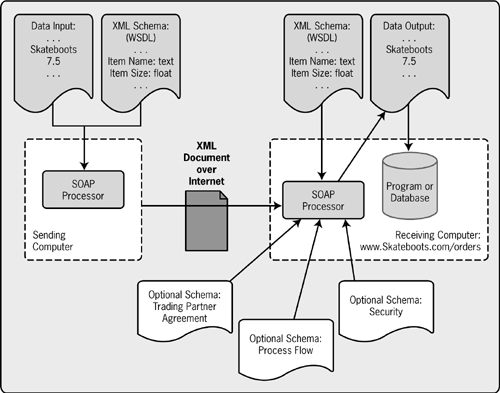
\includegraphics[width=250px]{WebServiceFuncionamento}
						\caption{Figura 1.1 - Web services use XML documents and transform them into and out of programs}
					\label{fig:WebServiceFuncionamento}
				\end{center}
			\end{figure}
		
			O processador de SOAP do computador de envio transforma os dados de seu formato nativo, para os tipos de dados do schema XML predefinido, contidos no arquivo WSDL, para texto, ponto flutuante, e outros, utilizando para isso tabelas de mapeamento. As tabelas de mapeamento associam os tipos de dados nativos com os seus correspondentes tipos de dados do schema XML. (Padrão de mapeamento são amplamente disponíveis para Java, Visual Basic, CORBA e outros sistemas dos tipos comumente usados. Muitas ferramentas de mapeamento XML estão disponíveis para definir mapeamentos personalizados ou especiais.) O processador SOAP do computador receptor realiza a transformação em sentido inverso, mapeando do schema XML, os tipos de dados correspondentes aos tipos de dados nativos.
		
			A URL, em uso generalizado na web, aponta para um endereço TCP (Transmission Control Protocol) que contém um recurso web, um Web Service schema contidos em arquivos acessíveis através da Internet  para download. Os Web Services disponíveis em um determinados endereços da Internet são identificados dentro de um arquivo público WDSL que pode ser baixado para o computador de envio e usado para gerar as mensagens. As Companhias também podem postar uma listagem no diretório público UDDI, apontando para o mesmo arquivo WSDL, para que clientes possam descobrir a empresa através do serviço UDDI. Em geral, quem quiser interagir com os Web Services deve encontrar uma maneira de obter e usar esse arquivo WSDL especial para gerar as mensagens.
		
		
\section{Implementação}

%Falar sobre a implementação do sistema, no caso falar como o Web services foi criado e afins
\lstset{ 
	language=php,               
	breaklines=true,                
	breakatwhitespace=false,        
	basicstyle      = \small\ttfamily,
	  keywordstyle    = \color{dkblue},
	  stringstyle     = \color{red},
	  identifierstyle = \color{dkgreen},
	  commentstyle    = \color{gray},
	  emph            =[1]{php},
	  emphstyle       =[1]\color{black},
	  emph            =[2]{if,and,or,else},
	  emphstyle       =[2]\color{dkyellow},
	  emph            =[3]{as,new,public,function,return,class,private,null,extends},
	  emphstyle       =[3]\color{dkblue},
	captionpos=b,
	numbers=left,                   % where to put the line-numbers
		numberstyle=\tiny\color{gray},  % the style that is used for the line-numbers
     stepnumber=1       
}

	
	Para a demostração da implementação de um web services, foi desenvolvida uma aplicação de agenda telefônica com servidor(web services) em linguagem de programação PHP junto ao \emph{Zend Framework} e no lado do cliente, uma aplicação android desenvolvida com \emph{PhoneGap} e framework javascript \emph{JQuery Mobile}.
	
	\subsection{Aplicação Servidor}

	Para a criação de um web service, utilizamos a classe do zend framework chamada Zend\_Soap\_Server que fornece toda funcionalidade de um web services no protocolo SOAP. Na listing \ref{listing:CriacaoWebServices}, temos a instanciação da classe e a configuração do web service, onde passamos um vetor com a versão do protocolo SOAP para 1.2, url do web service e codificação de caracteres. Logo em seguida é informada a url do WSDL e a classe que possui os serviços que serão disponibilizados. E finalmente o método \emph{handle()} para inicializar o web services.
	
	\lstinputlisting[language=PHP,caption={Criação de Web Services},label={listing:CriacaoWebServices}]{start_web_services_server.php}
	
	Para quem for usar o web services sabia as operações que possam ser realizadas, utilizamos o WSDL para descrever os serviço da API em detalhes. Foi utilizada a classe Zend\_Soap\_AutoDiscover que permite detectar automaticamente e realizar o mapeamento do da classe de serviço. Na listing \ref{listing:GeracaoWSDL}, verificamos se existe algum pedido de WSDL por parâmetro GET, caso exista ocorre a instanciação da classe AutoDiscover que faz a leitura da classe de modelo por meio de \emph{reflection} e gera o mapeamento WSDL.
	
	\lstinputlisting[language=PHP,caption={Geração do WSDL},label={listing:GeracaoWSDL}]{web_services_wsdl.php}
	
	Na classe de serviço, foi adicionado as operações disponíveis do web service para adicionar, remover e listar os contatos da agenda telefônica como mostrado na listing \ref{listing:ClasseServicos}.
	
	\lstinputlisting[language=PHP,caption={Classe de Serviços},label={listing:ClasseServicos}]{classe_servico.php}
	
	\subsection{Aplicação Cliente}
	
	No cliente, foi desenvolvida uma aplicação utilizando \emph{PhoneGap} e \emph{JQuery Mobile}. O PhoneGap permite o desenvolvimento de aplicações móveis para \emph{iOS, Android, Blackberry, Windows Phone, Palm WebOS, Bada} e \emph{Symbian} utilizando simplesmente: \emph{HTML, CSS} e \emph{Javascript}\cite{PHONEGAPSITE}.
	
	\emph{JQuery Mobile} fornece um sistema de interface unificado baseado em HTML5 para todas as populares plataformas.\cite{JQUERYMOBILESITE}
	
	\lstinputlisting[language=php,caption={Classe Cliente de Webservice},label={listing:ClasseClienteWebservice}]{classe_cliente.js}
	
	\lstinputlisting[language=html,caption={Template SOAP},label={listing:TemplateSOAP}]{template_soap.html}

\section{Como Utilizar}
	
	Eclipse
	\url{http://www.eclipse.org/downloads/packages/eclipse-ide-java-ee-developers/junor}  
	
	SDK do Android 
	\url{http://developer.android.com/sdk/installing/installing-adt.html}
	 
	Xampp para PHP 5.4
	\url{ http://www.apachefriends.org/pt_br/xampp-windows.html}
	
	
\section{Conclusão}
	Então podemos concluir que... cri cri cri


%\end{document}  % This is where a 'short' article might terminate

%
% The following two commands are all you need in the
% initial runs of your .tex file to
% produce the bibliography for the citations in your paper.
\bibliographystyle{abbrv}
\bibliography{sigproc}  % sigproc.bib is the name of the Bibliography in this case
% You must have a proper ".bib" file
%  and remember to run:
% latex bibtex latex latex
% to resolve all references
%
% ACM needs 'a single self-contained file'!
%
%APPENDICES are optional
%\balancecolumns
%\appendix
%Appendix A
%\section{Headings in Appendices}
%The rules about hierarchical headings discussed above for
%the body of the article are different in the appendices.
%In the \textbf{appendix} environment, the command
%\textbf{section} is used to
%indicate the start of each Appendix, with alphabetic order
%designation (i.e. the first is A, the second B, etc.) and
%a title (if you include one).  So, if you need
%hierarchical structure
%\textit{within} an Appendix, start with \textbf{subsection} as the
%highest level. Here is an outline of the body of this
%document in Appendix-appropriate form:
%\subsection{Introduction}
%\subsection{The Body of the Paper}
%\subsubsection{Type Changes and  Special Characters}
%\subsubsection{Math Equations}
%\paragraph{Inline (In-text) Equations}
%\paragraph{Display Equations}
%\subsubsection{Citations}
%\subsubsection{Tables}
%\subsubsection{Figures}
%\subsubsection{Theorem-like Constructs}
%\subsubsection*{A Caveat for the \TeX\ Expert}
%\subsection{Conclusions}
%\subsection{Acknowledgments}
%\subsection{Additional Authors}
%This section is inserted by \LaTeX; you do not insert it.
%You just add the names and information in the
%\texttt{{\char'134}additionalauthors} command at the start
%of the document.
%\subsection{References}
%Generated by bibtex from your ~.bib file.  Run latex,
%then bibtex, then latex twice (to resolve references)
%to create the ~.bbl file.  Insert that ~.bbl file into
%the .tex source file and comment out
%the command \texttt{{\char'134}thebibliography}.
%% This next section command marks the start of
%% Appendix B, and does not continue the present hierarchy
%\section{More Help for the Hardy}
%The acm\_proc\_article-sp document class file itself is chock-full of succinct
%and helpful comments.  If you consider yourself a moderately
%experienced to expert user of \LaTeX, you may find reading
%it useful but please remember not to change it.
%\balancecolumns
%% That's all folks!
\end{document}
